\documentclass[12pt,utf8]{scrartcl}
\usepackage[ngerman]{babel}
\usepackage{hyperref}
\hypersetup{
	colorlinks=true,	
	linkcolor=blue,     
	citecolor=blue,     
	filecolor=blue,     
	urlcolor=blue     	
}
\usepackage{etoolbox}
\apptocmd{\UrlBreaks}{\do\-\do\%\do\.}{}{}
\usepackage[ngerman]{varioref}
\usepackage{amsmath,amssymb,latexsym,amsfonts,amsthm,amsbsy,qtree}
\usepackage{url}
\usepackage[printonlyused]{acronym}
\usepackage[utf8]{inputenc} 
\usepackage{graphicx}
\usepackage{float}
\usepackage{fancyhdr}
\usepackage{booktabs}
\usepackage{enumitem}
\usepackage[justification=centering]{caption}
\usepackage[numbers]{natbib}
\bibliographystyle{plainnat}
\usepackage{pdfpages}

\newcommand{\teilnehmerI}{Tom Dombeck}
\newcommand{\mattI}{4510671} 
\newcommand{\mailI}{todo@uni-bremen.de}
\newcommand{\teilnehmerII}{Andreas Schwarz}
\newcommand{\mattII}{4250572}
\newcommand{\mailII}{andreas4@uni-bremen.de}
\newcommand{\teilnehmerIII}{Lasse Warnke}
\newcommand{\mattIII}{4515161}
\newcommand{\mailIII}{lwarnke@uni-bremen.de}
\newcommand{\thisgroup}{A01}
\newcommand{\abgabedatum}{23.12.2018}
\newcommand{\nummer}{2}
\newcommand{\thema}{Integrierte Anwendungssysteme, Big Data}
\newcommand{\thistutor}{Tim Haß}
\newcommand{\thissemester}{WiSe 2018/19}
\newcommand{\thiscourse}{Wirtschaftsinformatik 1}
\newcommand{\thisshortcourse}{WI1}

\pagestyle{fancy}
\fancyhead{} 												
\fancyhead[LO,RE]{\thissemester \\ \thisshortcourse} 
\fancyhead[RO,LE]{TutorIn: \thistutor \\ Gruppe: \thisgroup }
\fancyfoot{} 											
\cfoot{\thepage} 										
\setlength{\headsep}{2cm} 								

\begin{document}
\begin{titlepage}
	\vspace*{\baselineskip}		
	\centering					
	\LARGE							
	\thiscourse \\ 					
	\vspace{1cm}					
	{\Huge 							
	\textbf{Abgabe \nummer: \thema}} \\ 
	\vspace{1.5cm} 					
	TutorIn: \thistutor \\ 		
	\abgabedatum \\ 				
	\vfill 							
	Gruppe: \thisgroup \\ 			
	\vspace{.5cm} 					
	\large 							
	\begin{tabular}{c|c|c} 		
	\teilnehmerI	& \teilnehmerII & \teilnehmerIII \\ 
	\mattI	& \mattII &  \mattIII\\ 
	\mailI	& \mailII & \mailIII \\ 
	\end{tabular} 
\end{titlepage}

\thispagestyle{empty}
\tableofcontents
\newpage
\setcounter{page}{1}

\section*{Aufgabe 2.1}
\addcontentsline{toc}{section}{Aufgabe 2.1}
\subsection*{\label{sub:thema}1. Probleme der dezentralen Lösung}
\addcontentsline{toc}{subsection}{1. Probleme der dezentralen Lösung}

Um die Probleme welche das dezentrale System dem Bremer Polizeipräsidium verursacht zu verstehen muss man erstmal seinen Aufbau kennen. Aktuell besitz jede Abteilung, oder zumindest jede genannte, ihr eigenens IT-System. Das bedeuted entweder ein stark personalisiertes oder sogar selbst entwickeltes System. 

Diese Insellösungen sorgen für eine ganze Menge Probleme. Vor allem wenn man das jetzige System mit einem zentralisierten IT-System vergleicht. 
Das erste und offensichtlichste Problem ist die kompatibilität der einzelnen Systeme. Also der Datenaustasch zwischen den einzelene Abteilungen des Polizeipräsidiums. Durch die wahrscheinlich stark unterschiedlichen Systeme ist es nicht unbedingt gewährleistet das diese miteinander kompatibel sind und dadurch effizient Daten zwischen den einzelnen Abteilungen ausgetauscht werden können (wenn dies überhaupt ohne Umweg möglich ist).

Dies führt gleichzeitig natürlich auch zu einem erhöhten Administrationsaufwand um die unterschiedlichen Systeme am laufen zu halten. Da viele verschiedenen IT-Systeme gibt wird eine größere Anzahl an Administratoren gebraucht welche sich auch noch  mit vielen verschiedenen Systemen auskennen müssen. Dies führt wahrscheinlisch zu höheren Personalkosten als auch zu mehr Ausfällen als wenn es ein zentrales IT-System geben würde.

Ein weiterer nicht zu vernachlässigender Punkt ist die Sicherheit welche durch die große Anzahl an verschiedenen System natürlich ebenfalls beeinträchtigt ist. Im vergleich zu einem zentralen System ist es bei den vielen verschiedenen Abteilungssystemen schwieriger einen einheitlichen Sicherheitsstandard einzuhalten.

Ein Problem welches schon bei der Administration angesprochen wurde ist die Ausfallsicherheit eines solchen dezentralen Systems. Durch die verschiedenen Syteme und dadurch auch verteilte Aufmerksamkeit der Administratoren auf dei verschiedenen Syteme ist es natürlich schwieriger eine große Anzahl von Systemen 24/7 am laufen zu halten als ein Sytem welches die ungeteilte Aufmerksamgeit aller Administratoren genießt.\cite{APariConsulting}


\subsection*{\label{sub:thema}2. Sytemlandkarte mit Sollkonzept}
\addcontentsline{toc}{subsection}{2. Sytemlandkarte mit Sollkonzept}

Grundlegend werden bei deisem Konzept alle Abteilungen mit allen verbunden. Es entsteht ein zentrales Serversystem und eine zentrale Datenbank oder zumindest zetral zugängliche Datenbanken für die normal anfallenden Daten. Für besonders vertrauliche Daten wie z.B. Einstzpläne oder die Liste der aktuell sich in Polizeigewahrsam befindenden Personen wird eine externe Datenbank angelegt auf welche nur von den jeweiligen Abteilungen zugegriffen werden kann.

Durch die zentrale Infrastruktur um die zentrale Datenbank herum können Schnittstellen zwischen den einzelnen Abteilungen relativ einfach realisiert werden. Dies ist auch wichtig, da es zwischen so gut wie allen Abteilungen auch Schnittstellen benötigt werden. 

So müssen Einsatzleitung, Budgetverwaltung und Personalverwaltung auf nahezu jede andere Abteilung zugreifen.

Die Einstzleitung muss ständig einen Überblick über alle zur verfügung stehenden Mittelhaben um Einsätze effizient und ohne andere Abteilungen dabei zu stören planen können. So mussen sie z.B auf die Personalverwaltung zugreifen können um um die aktuell zur verfügung stehende Zahl an Kräften einschätzen zu können. Ähnliches gilt auch für den Zugriff auf die Fuhrparkverwaltung um die Zahl an zur Verfügung stehenden Einsatzwagen einschätzen zu können.

Die Budgetverwaltung muss mehr oder weniger auf alle Abteilungen zugreifen können um in der Lage zu sein das zur Verfügung stehende Budget sinvoll auf die einzelen Abteilungen aufzuteilen. So nuss z.B. ständig bekannt sein wieviel Personal vorhanden ist und in Welcher Gehaltsstufe sich diese befinden. Das gleiche gilt auch bei der Einkaufsabteilung. Von dieser muss ständig bekannt sein wieviel Geldmittel benötigt werden und auch in die andere Richtunge wieviel Geld zur Verfügung steht. Ähnliches gilt auch für die anderen Abteilungen da es ja in jedem Fall um die für die jeweilige Abteilung zur Verfügung stehenden und benötigten Geldmittel geht.

Desweiteren muss ständig durch die Materialverwaltung der aktuelle Lagerbestand bekannt sein damit der Einkauf die jeweilige Sache im Falle einer Knappheit neu beschaffen kann. Genau so wichtig ist der Kontakt mit der Budgetabteilung um Genhmigung der benötigten Geldmittel möglichst schnell und effizient zu ermöglichen.

Die Personalverwaltung benötigt einen Überblick über die aktuelle Personalsituation. Dafür braucht sie Zugriff auf die Einsatzplanung um die Zahl der sich aktuell im Einsatz befindenden Kräfte zu bekommen sowie Zugriff auf das Reviermanagement für die Zahl der andersweitig eingeplanten Personen. Desweitern muss sie mit der Bewerbungsabteilung komunizieren können um die Einstellung und Ausbilding neuer Polizisten möglichst effizient managen zu können.

Allgemein kann man sagen, dass alle "standard"-Daten, also Daten wie verfügbares Geld, Personalstärke und Lagerstand, in die Datenbank abgelegt werden sollten damit diese von den Abteilungen genutzt werden können. 
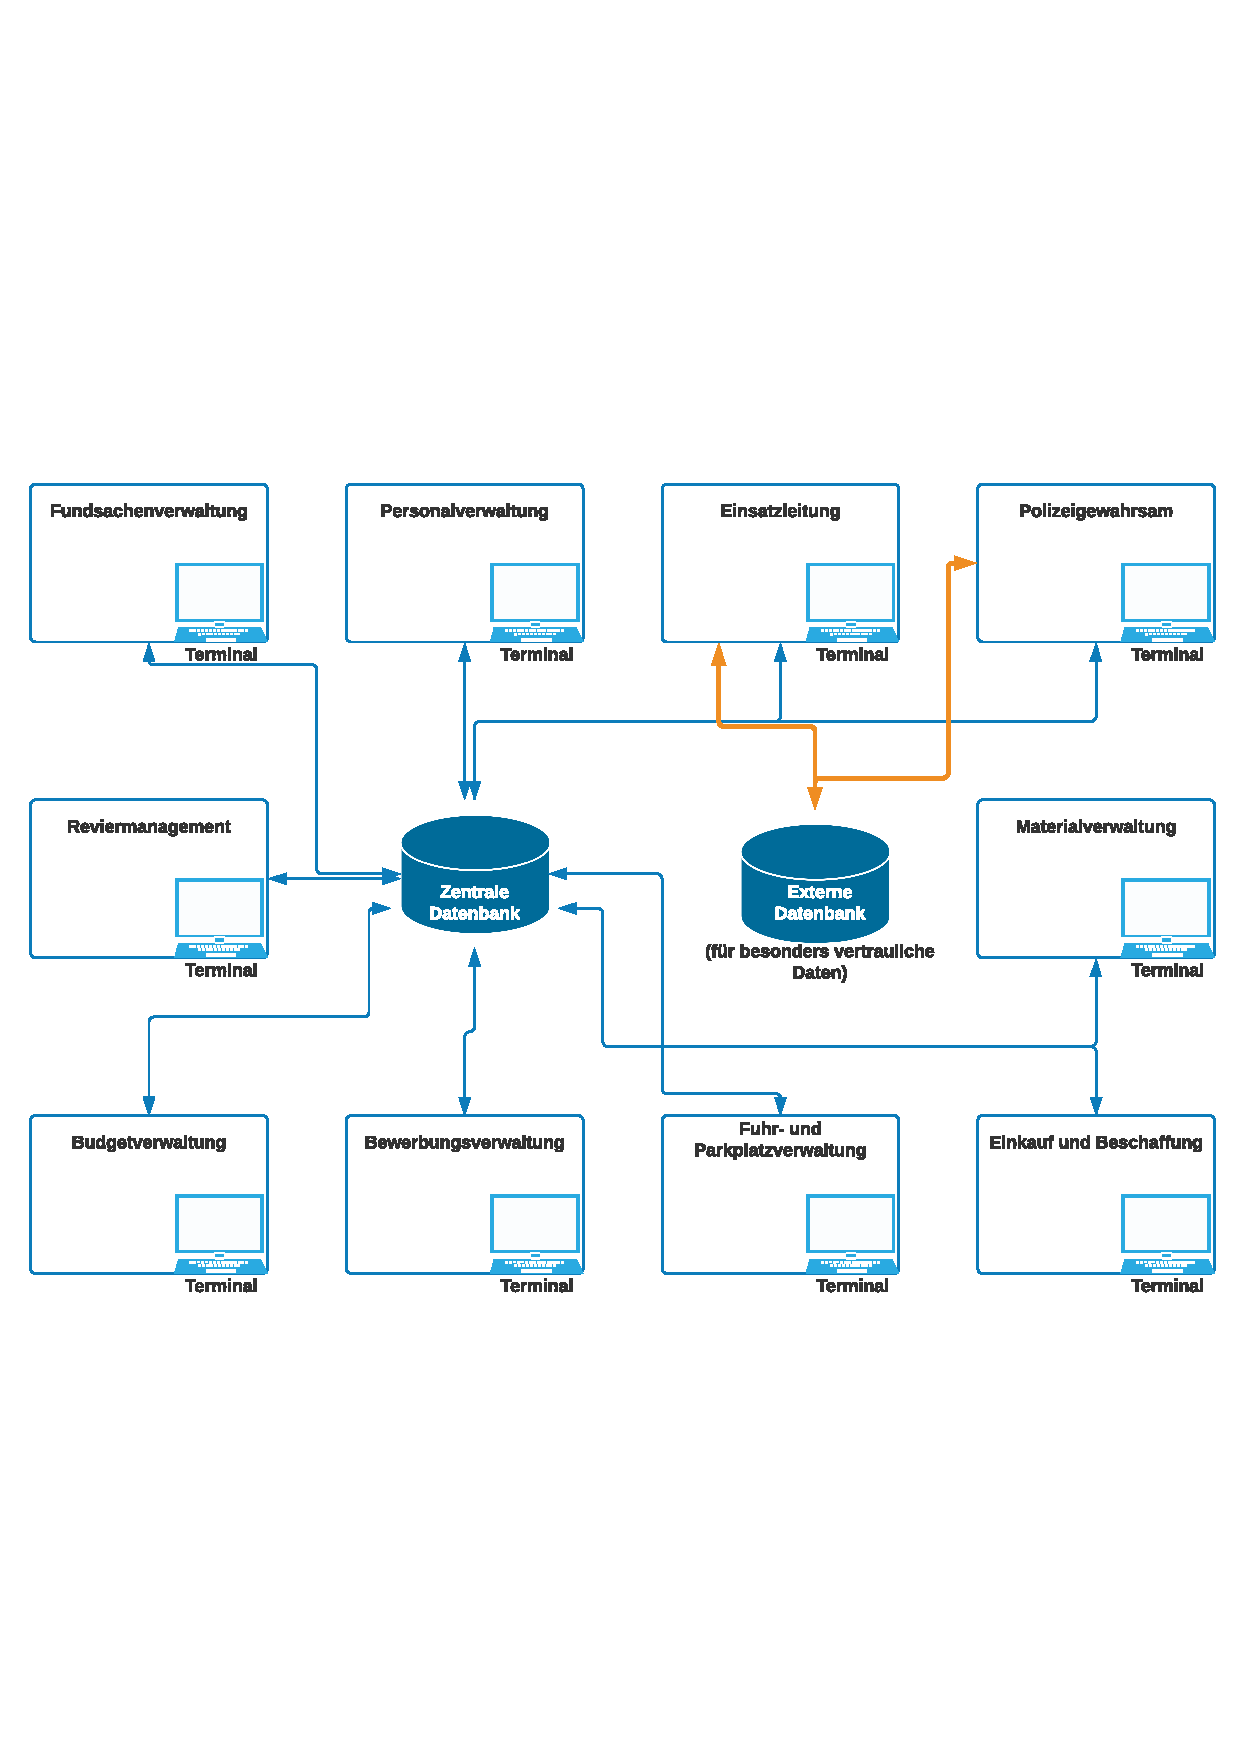
\includepdf[pages=1]{NetworkDiagram.pdf}



\subsection*{2.1.3}\label{Aufgabe 2.1.3}
\addcontentsline{toc}{subsection}{3. ERP-Module für Polizei Bremen}

ERP-Systeme sind modular aufgebaut und somit an einzelne Kunden besser individuell anpassbar. Moderne ERP-Systeme umfassen oft eine große Zahl an Funktionsbereichen oder Modulen. 

- Fundsachenverwaltung -> 
- Personalverwaltung -> Personalwirtschaft
- Einsatzleitung -> 
- Materialverwaltung -> 
- Polizeigewahrsam -> 
- Reviermanagement -> 
- Budgetverwaltung -> Finanz- und Rechnungswesen
- Bewerbungsverwaltung -> 
- Fuhr- und Parkplatzverwaltung -> 
- Einkauf und Beschaffung -> 

\subsection*{2.1.4}
\addcontentsline{toc}{subsection}{4. Einführung eines ERP-Systems für die Polizei Bremen}

Es gibt verschiedene Herangehensweisen um ein ERP-System neu in ein Unternehmen einzuführen. Man kann entweder schrittweise vorgehen oder man macht einen sogenannten "Big Bang", bei dem man das komplette System an einem Stichtag einführt. Natürlich haben beide Varianten ihre Vor- und Nachteile. So müssen bei einer schrittweisen Einführung die alten Systeme und das neue ERP-System temporäre Schnittstellen haben, damit alle Systeme weiterhin funktionieren. Dies ist bei einem "Big Bang" natürlich nicht nötig, da alle alten Systeme auf einen Schlag ersetzt werden. Auf der anderen Seite muss die Umstellung auf ein anderes System natürlich vorbereitet werden. Alle Mitarbeiter müssen z.B. geschult und mit dem neuen System vertraut gemacht werden. Dies ist natürlich einfacher, wenn man ein System nur nach und nach z.B. an verschiedenen geographischen Standorten oder nach Modulen geordnet einführt, da man so eine kleinere Anzahl an Leuten zur gleichen Zeit schulen muss\cite{Jacob2008}. 

Für die Polizei Bremen würden wir ein schrittweise eingeführtes ERP-System empfehlen, weil es sich mit rund 2.500 Angestellten um ein recht großes "Unternehmen" handelt, das zudem weit über das Land Bremen verstreut ist\cite{PolizeiBremen}. 

Da alle Geschäftsprozesse, die unterstützt werden sollen, und somt auch alle ERP-Module, die für die Polizei Bremen in Frage kommen, schon geklärt sind (siehe Aufgabe 2.1.2 und 2.1.3), ist der erste Schritt auf dem Weg zur Einführung eines ERP-Systems schon gemacht. 

\newpage
\begin{flushleft}
\addcontentsline{toc}{section}{Literaturverzeichniss}
\bibliography{Literaturdatenbank}
\end{flushleft}
\end{document}
